\documentclass[11pt,a4paper]{article}
\usepackage[utf8]{inputenc}
\usepackage[T1]{fontenc}
\usepackage{amsmath,amssymb}
\usepackage{booktabs}
\usepackage{graphicx}
\graphicspath{{figure-p4/}}
\usepackage{geometry}
\usepackage{times}
\usepackage{array}
\usepackage[hidelinks]{hyperref}
\geometry{margin=2.5cm}
\setlength{\parindent}{0pt}
\setlength{\parskip}{0.4em}
\linespread{1.0}

% ============================================================
% Paper 4 - XAI untuk NIDS (VERSI JICTRA, English, LaTeX).
% Semua ANGKA dari eksperimen nyata (notebook_xai/01-03 di AWS SageMaker;
% CIC-IDS2017 MachineLearningCSV mentah -> CSE-CIC-IDS2018). Pipeline bebas-kebocoran,
% TANPA Semantic Feature Mapping. Gambar: PNG dari notebook 04_figures (figure-p4/).
% ============================================================

\title{\textbf{Explainable AI for Network Intrusion Detection:
Diagnosing and Repairing Cross-Dataset Generalization Failure
on a Leakage-Free Pipeline}}

\author{First Author\thanks{Corresponding author.},
\quad Second Author, \quad Third Author \\[0.3em]
\normalsize Department of Informatics and Computer Engineering, \\
\normalsize Politeknik Elektronika Negeri Surabaya (PENS), Surabaya, Indonesia \\
\normalsize \texttt{author1@pens.ac.id; author2@pens.ac.id; author3@pens.ac.id}}

\date{}

\begin{document}
\maketitle

\begin{abstract}
\noindent Machine-learning network intrusion detection systems (NIDS) often appear nearly
perfect under within-dataset evaluation yet collapse on datasets with different attack
compositions and recording conditions. This paper presents a diagnosis and repair of
cross-dataset generalization failure using a leakage-free pipeline, with CIC-IDS2017 as the
reference dataset and CSE-CIC-IDS2018 as the transfer target, both extracted with
CICFlowMeter and aligned by feature-name intersection only (no semantic feature mapping).
Two classifiers, XGBoost and Random Forest, are trained on the reference and transferred to
the target without retraining. Within-dataset performance is high (Matthews correlation
coefficient, MCC, of 0.955 and 0.979). Across datasets, MCC at the default threshold
collapses to 0.067 and 0.175 with near-zero attack recall, while weighted-F1 remains
misleadingly high. Unlike prior work that stops at diagnosis, we (i) separate ranking
failure from thresholding failure: cross-dataset AUC stays above chance (0.779 for XGBoost)
and threshold calibration lifts MCC to 0.498, whereas for Random Forest calibration reaches
only 0.403; and (ii) repair detection with minimal few-shot calibration, where only 1\% of
target labels raises MCC to 0.663 (XGBoost) and 0.871 (Random Forest), and above 0.96 in
the reverse direction. SHAP is read in a condition-aware manner: feature-ranking stability
(Spearman 0.72 between failed and repaired models) does not imply transferability. The
findings reinforce reporting MCC, per-class recall, threshold calibration, and cross-dataset
validation in NIDS research.

\medskip
\noindent\textbf{Keywords:} explainable AI; network intrusion detection; cross-dataset
generalization; threshold calibration; few-shot calibration; SHAP; Matthews correlation
coefficient.
\end{abstract}

\section{Introduction}
Digital transformation widens the network attack surface and raises the need for reliable
NIDS. Machine-learning detectors are widely used because they learn traffic patterns from
benchmark datasets such as CIC-IDS2017 \cite{sharafaldin} and CSE-CIC-IDS2018; surveys
document a broad range of such detectors \cite{buczak,shone,wu}. High within-dataset accuracy,
however, does not guarantee operational reliability on a different environment
\cite{dhooge,cantone}. Layeghy and Portmann \cite{layeghygen} show that NIDS models that
are near-perfect on synthetic benchmarks often fail to generalize to other networks, as
differing infrastructure and protocols induce covariate and concept shift; transfer-learning
surveys for IDS \cite{kheddar} underline domain adaptation as essential when target-domain
labels are scarce.

Two methodological problems stand out. First, \emph{data leakage} arises when feature
selection, standardization, or oversampling is performed before the train-test split,
producing over-optimistic estimates. Second, \emph{feature-schema compatibility does not
imply distribution compatibility}: even when feature names and counts match (both datasets
use CICFlowMeter), feature statistics can differ because of different attack compositions
and recording conditions; several works further document label and feature-quality
issues in these datasets \cite{engelen,rosay,lanvin,liu,catillo} and question how well
synthetic benchmarks reflect real traffic \cite{layeghy}. Credible cross-dataset evaluation
therefore calls for a leakage-aware pipeline and, ideally, bidirectional transfer analysis
so that reliability is not judged from a single direction.

A prior study by the authors \cite{martono} diagnosed this phenomenon but had three
limitations that this paper addresses: (1) it \emph{stopped at diagnosis}, reporting failure without a repair;
(2) it \emph{conflated two failure modes}, reading an MCC of zero purely as distribution
shift even though a varying AUC indicated a partial thresholding problem; and (3) it
computed SHAP without regard to model condition, so interpretations on a model whose attack
recall was zero were fragile. Explainability methods such as SHAP \cite{lundberg} and
LIME \cite{ribeiro} are increasingly applied to NIDS \cite{arreche,gaspar,wang,mohale,alabbaadi},
yet their interpretations are rarely tied to whether the model actually detects attacks.

To address these limitations, this paper contributes a leakage-free pipeline for binary
cross-dataset IDS experiments between CIC-IDS2017 and CSE-CIC-IDS2018 (in both directions)
that aligns features by name intersection without semantic feature mapping. On this
pipeline we separate \emph{ranking failure} (measured by AUC/PR-AUC) from
\emph{thresholding failure} (MCC at the default threshold) and then apply threshold
calibration; in contrast to deep domain-adaptation methods such as DI-NIDS and DANN
\cite{layeghydi}, which require a heavy network stack and ample target data, our repair is
a lightweight few-shot calibration that uses only a small fraction of target labels and is
reported with multi-seed confidence intervals. We further compare XGBoost and Random Forest
under an identical protocol to test whether the failure-then-repair pattern is
algorithm-general, and we interpret the models with a condition-aware SHAP analysis that
contrasts the failed and repaired models for both algorithms, showing that feature-ranking
stability does not by itself imply cross-dataset transferability.

\section{Method}
\subsection{Datasets and Experimental Scope}
Experiments use two CICFlowMeter benchmark datasets: \textbf{CIC-IDS2017} as the reference
(training) dataset, with mixed attacks (brute force, DoS, DDoS, web attack, infiltration,
botnet, port scan), and \textbf{CSE-CIC-IDS2018} as the cross-dataset target, whose attack
composition and recording conditions differ. All labels are mapped to a binary scheme
(benign/normal $=0$, attack $=1$). To control computation, each source file is
stratified-subsampled to at most 100{,}000 rows. Table~\ref{tab:data} summarizes the data
after cleaning and splitting.

\begin{table}[htbp]
\centering
\caption{Dataset summary after preprocessing and stratified subsampling.}
\label{tab:data}
\footnotesize
\begin{tabular}{lrrrrr}
\toprule
Dataset & Sampled & Train (80\%) & Test (20\%) & Shared feat. & \%Attack \\
\midrule
CIC-IDS2017 (ref)       & $799{,}989$ & $639{,}991$ & $159{,}998$ & $76$ & $19.26$ \\
CSE-CIC-IDS2018 (target)& $999{,}987$ & $799{,}989$ & $199{,}998$ & $76$ & $23.83$ \\
\bottomrule
\end{tabular}
\end{table}

\subsection{Leakage-Free Pipeline}
All fitting operations use training data only. The processing order is: (1) column and
label normalization (whitespace/BOM cleanup, alias mapping across CICFlowMeter releases,
binary label mapping); (2) data cleaning (drop metadata such as IP, port, protocol,
timestamp, and flow id; remove duplicates; convert infinities to NaN; drop dominantly
missing columns; impute remaining numeric missing values with the \emph{training} median);
(3) feature-schema alignment by \emph{name intersection} (no semantic mapping, no zero
fill), in contrast to standardized feature-set efforts \cite{sarhan}; (4) stratified 80/20 split; (5) feature selection, \texttt{StandardScaler}, and
SMOTE \cite{chawla} fitted \emph{only} on training data; all models use scikit-learn
\cite{pedregosa}. The pipeline is illustrated in
Figure~\ref{fig:pipeline}. For cross-dataset evaluation, the model, scaler, and selected
feature list from the reference are applied directly to the target, measuring transfer
rather than re-adaptation. All notebooks run on AWS SageMaker; raw CSVs are synced from
Amazon S3 and result artifacts uploaded back.

\begin{figure}[htbp]
\centering
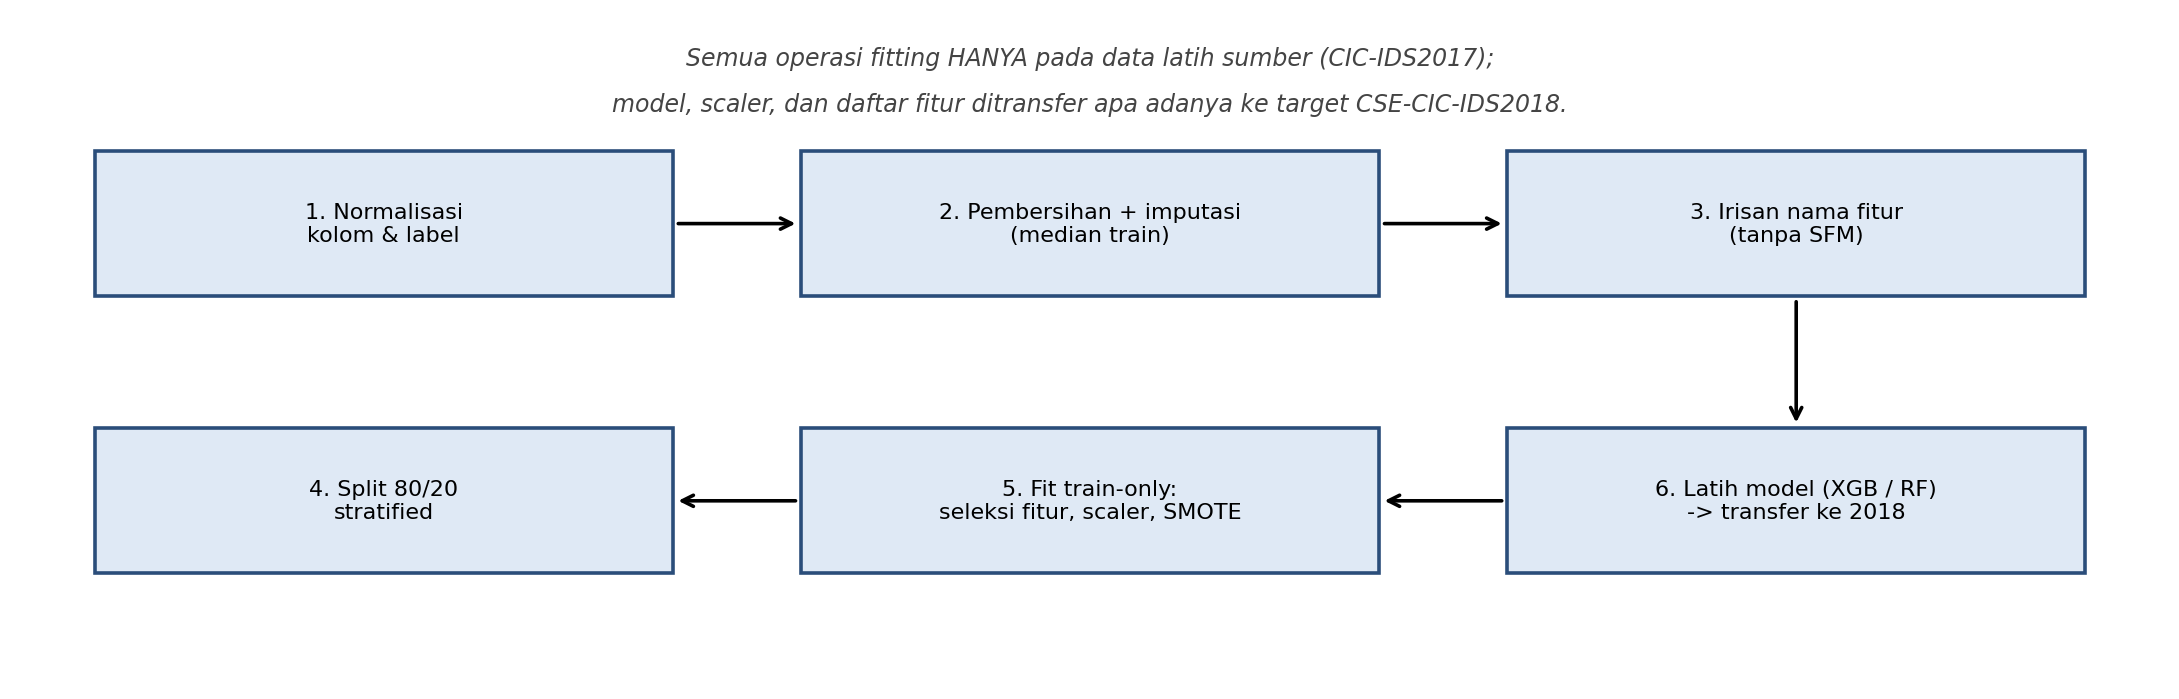
\includegraphics[width=0.95\textwidth]{figure-p4/fig1_pipeline.png}
\caption{Leakage-free cross-dataset evaluation pipeline. All fitting (median imputation,
feature selection, standardization, SMOTE) uses the source training split only; the fitted
model, scaler, and feature list are then transferred unchanged to the target dataset.}
\label{fig:pipeline}
\end{figure}

\subsection{Classification Models}
Related NIDS studies span tree ensembles and boosting \cite{breiman,chen,ke,husain} and
UNSW-NB15-based detectors \cite{moustafa15,moustafa16}. Two models are compared under an
identical pipeline: \textbf{XGBoost} (\texttt{max\_depth}=8,
\texttt{learning\_rate}=0.1, \texttt{n\_estimators}=200,
\texttt{subsample}=\texttt{colsample\_bytree}=0.8) and \textbf{Random Forest}
(\texttt{n\_estimators}=200, \texttt{max\_depth}=20). Random Forest parallels the reference
study; XGBoost represents modern gradient boosting common in IDS.

\subsection{Evaluation Metrics}
We report accuracy, precision, recall (per class), weighted F1, AUC-ROC, PR-AUC, and MCC.
MCC is prioritized for cross-dataset evaluation because it accounts for TP/TN/FP/FN
simultaneously and remains informative under class imbalance \cite{chicco}. To separate
ranking failure from thresholding failure, threshold-independent AUC/PR-AUC are reported
together with MCC and attack recall at both the default and a calibrated threshold. Prior cross-dataset
and unsupervised-generalization studies motivate this emphasis \cite{verkerken}, as does
work on domain adaptation \cite{sun} and interpretable modeling \cite{molnar}.

\subsection{Threshold Calibration and Few-Shot Repair}
The decision threshold is re-selected on a small target calibration subset (maximizing MCC)
to test whether part of the ``failure'' is merely a threshold artifact. For few-shot repair,
a small fraction of target labels (0\%, 1\%, 5\%, 10\%) is added to training, and the gain
in MCC and attack recall is measured.

\subsection{Explainability with SHAP}
TreeSHAP provides global feature importance for each transfer direction. Features are ranked
by mean absolute SHAP value; rank agreement is measured with Spearman correlation.
Crucially, SHAP is computed in a \emph{condition-aware} way on both the failed model (before
repair) and the repaired model (after few-shot), to test whether feature stability equals
transferability.

\section{Results and Discussion}
\subsection{Within-Dataset Performance}
On within-dataset CIC-IDS2017 (Table~\ref{tab:within}), both models score high. These
near-perfect scores must not be read as cross-environment readiness.

\begin{table}[htbp]
\centering
\caption{Within-dataset performance on CIC-IDS2017 (mean over 5 seeds).}
\label{tab:within}
\footnotesize
\begin{tabular}{lcc}
\toprule
Metric & XGBoost & Random Forest \\
\midrule
F1 (weighted) & $0.986$ & $0.993$ \\
MCC           & $0.955$ & $0.979$ \\
AUC-ROC       & $0.999$ & $1.000$ \\
Attack recall & $0.939$ & $0.998$ \\
\bottomrule
\end{tabular}
\end{table}

\subsection{Cross-Dataset Generalization}
Table~\ref{tab:cross} reports transfer in both directions. Despite near-perfect
within-dataset scores, cross-dataset MCC at threshold 0.5 collapses (0.067 and 0.175 for
CIC2017$\rightarrow$CIC2018) with attack recall near zero.

\begin{table}[htbp]
\centering
\caption{Cross-dataset evaluation (direct transfer, threshold 0.5, mean over 5 seeds).}
\label{tab:cross}
\footnotesize
\begin{tabular}{lllccccc}
\toprule
Model & Direction & Type & F1 & MCC & AUC & PR-AUC & Att.\ recall \\
\midrule
XGBoost & CIC2017 & Within & $0.986$ & $0.955$ & $0.999$ & --- & $0.939$ \\
XGBoost & CIC2017$\rightarrow$CIC2018 & Cross & $0.665$ & $0.067$ & $0.779$ & $0.619$ & $0.013$ \\
XGBoost & CIC2018$\rightarrow$CIC2017 & Cross & $0.759$ & $0.188$ & $0.684$ & $0.391$ & $0.119$ \\
RF & CIC2017 & Within & $0.993$ & $0.979$ & $1.000$ & --- & $0.998$ \\
RF & CIC2017$\rightarrow$CIC2018 & Cross & $0.687$ & $0.175$ & $0.573$ & $0.456$ & $0.056$ \\
RF & CIC2018$\rightarrow$CIC2017 & Cross & $0.868$ & $0.574$ & $0.863$ & $0.676$ & $0.474$ \\
\bottomrule
\end{tabular}
\end{table}

\subsection{Weighted-F1 vs MCC Discrepancy}
For CIC2017$\rightarrow$CIC2018, weighted-F1 stays high (0.665 and 0.687) while MCC collapses
and attack recall is 0.013--0.056: the model passes ``accuracy'' by predicting the dominant
benign class while barely detecting attacks. Figure~\ref{fig:f1mcc} contrasts the two
metrics. Weighted-F1 and accuracy alone are therefore inadequate for cross-dataset IDS;
MCC and per-class recall are mandatory.

\begin{figure}[htbp]
\centering
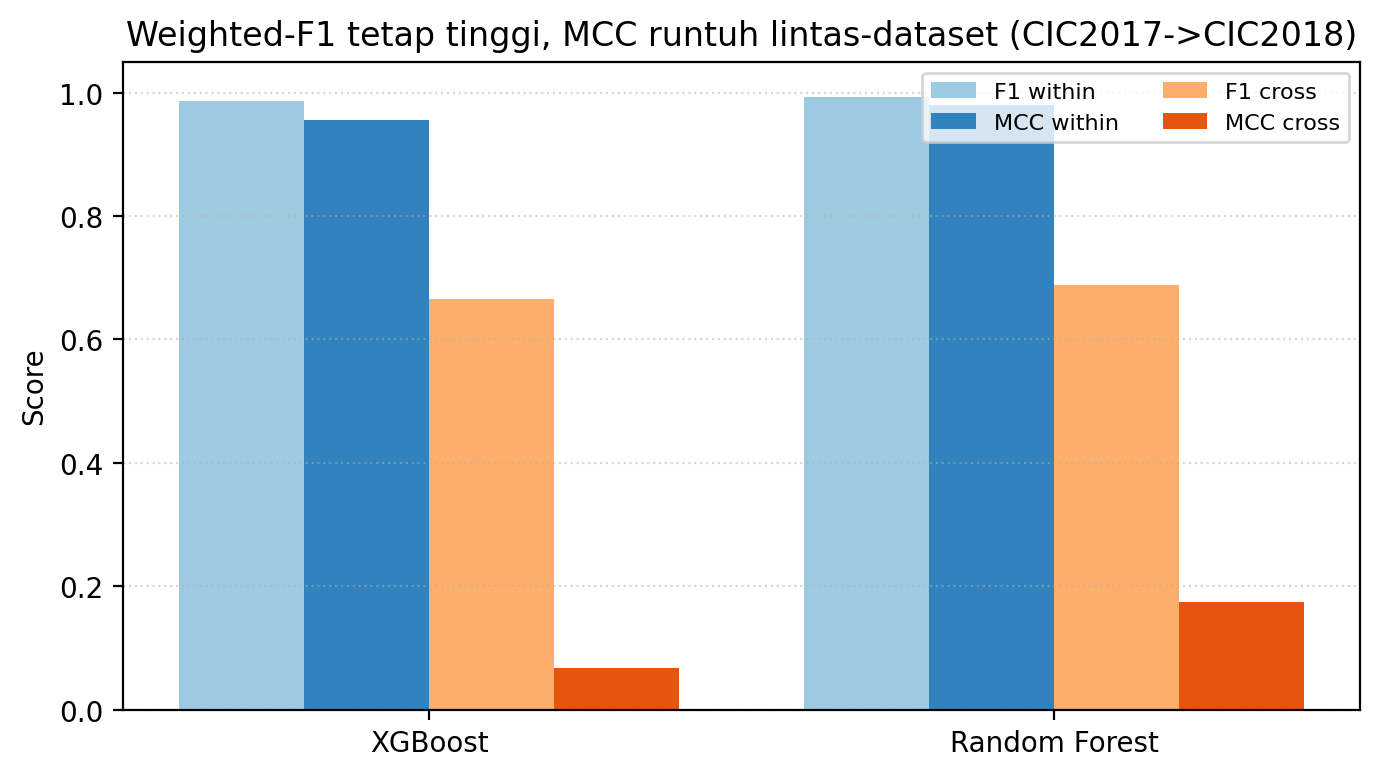
\includegraphics[width=0.8\textwidth]{figure-p4/fig2_f1_vs_mcc.png}
\caption{Weighted-F1 versus MCC, within-dataset against cross-dataset, for both models.
Weighted-F1 follows the dominant benign class, whereas MCC exposes the failure to separate
benign from attack across datasets.}
\label{fig:f1mcc}
\end{figure}

\subsection{Ranking vs Thresholding: Threshold Calibration}
A key finding: cross-dataset failure is not of a single kind. For XGBoost
CIC2017$\rightarrow$CIC2018, AUC remains 0.779 (well above the chance level of 0.5) even
though MCC@0.5 is only 0.067; recalibrating the decision threshold on a small target subset
raises MCC to 0.498 (Table~\ref{tab:thr}). The model can still rank attacks above benign,
so much of the ``failure'' is a threshold artifact. By contrast, for Random Forest in the
same direction AUC is only 0.573 (near chance), so calibration lifts MCC only to 0.403:
here the failure is one of ranking, not merely thresholding.

\begin{table}[htbp]
\centering
\caption{Effect of threshold calibration on the target (mean over 5 seeds).}
\label{tab:thr}
\footnotesize
\begin{tabular}{llcc}
\toprule
Model & Direction & MCC@0.5 & MCC@calibrated \\
\midrule
XGBoost & CIC2017$\rightarrow$CIC2018 & $0.067$ & $0.498$ \\
XGBoost & CIC2018$\rightarrow$CIC2017 & $0.188$ & $0.362$ \\
RF & CIC2017$\rightarrow$CIC2018 & $0.175$ & $0.403$ \\
RF & CIC2018$\rightarrow$CIC2017 & $0.574$ & $0.633$ \\
\bottomrule
\end{tabular}
\end{table}

\subsection{Few-Shot Recovery}
Adding only 1\% of target labels restores detection dramatically
(Table~\ref{tab:fewshot}, Figure~\ref{fig:fewshot}): for CIC2017$\rightarrow$CIC2018, MCC
rises from 0.067 to 0.663 (XGBoost) and from 0.175 to 0.871 (Random Forest); in the reverse
direction, from 0.188 to 0.969 and from 0.574 to 0.967. Larger budgets (5\%, 10\%) yield
diminishing gains. Recovery is consistent across both directions and both models, indicating
low-cost domain adaptation is a general, practical route.

\begin{table}[htbp]
\centering
\caption{Few-shot recovery: MCC per fraction of target labels (mean over 5 seeds).}
\label{tab:fewshot}
\footnotesize
\begin{tabular}{llcccc}
\toprule
Model & Direction & 0\% & 1\% & 5\% & 10\% \\
\midrule
XGBoost & CIC2017$\rightarrow$CIC2018 & $0.067$ & $0.663$ & $0.738$ & $0.813$ \\
XGBoost & CIC2018$\rightarrow$CIC2017 & $0.188$ & $0.969$ & $0.984$ & $0.986$ \\
RF & CIC2017$\rightarrow$CIC2018 & $0.175$ & $0.871$ & $0.882$ & $0.884$ \\
RF & CIC2018$\rightarrow$CIC2017 & $0.574$ & $0.967$ & $0.985$ & $0.989$ \\
\bottomrule
\end{tabular}
\end{table}

\begin{figure}[htbp]
\centering
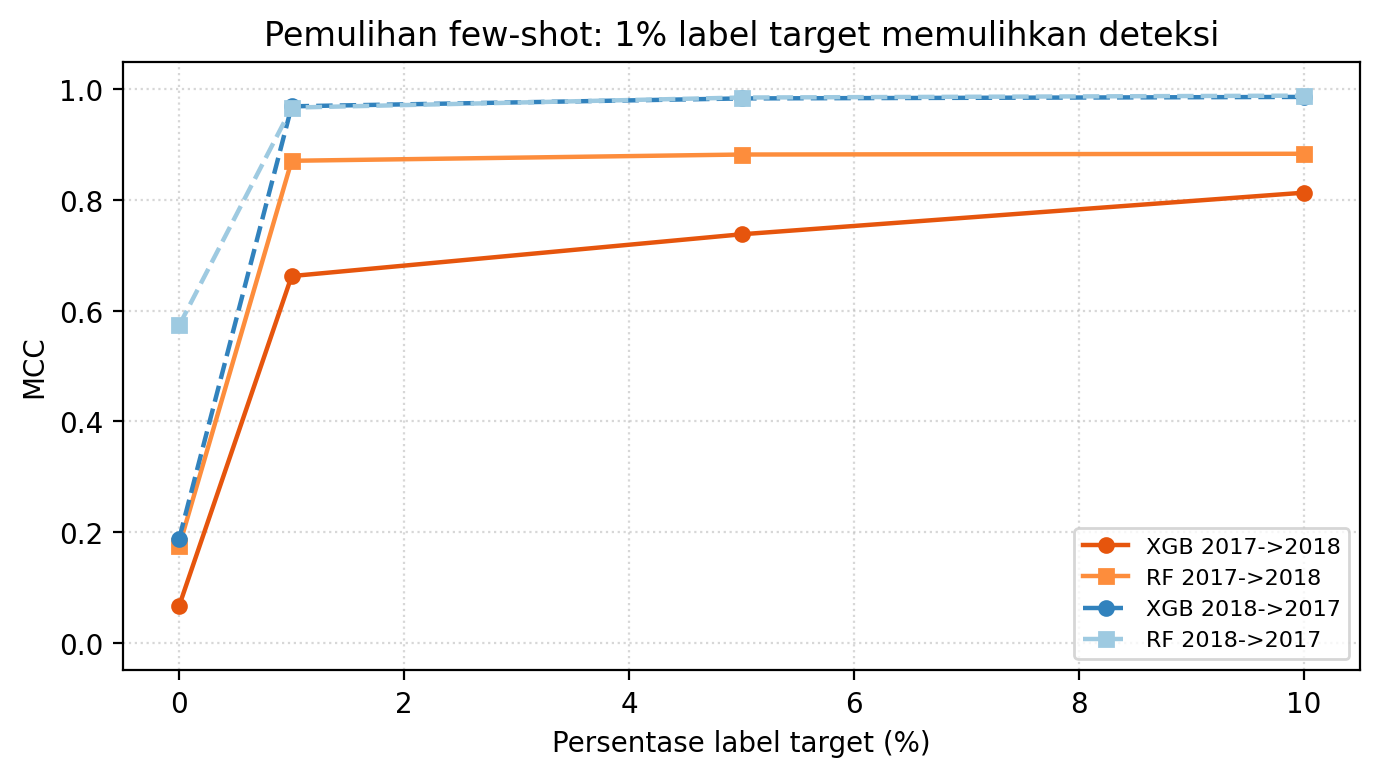
\includegraphics[width=0.8\textwidth]{figure-p4/fig3_fewshot.png}
\caption{Few-shot recovery curves (MCC versus fraction of target labels added) for both
models and both transfer directions. Even 1\% of target labels restores most achievable
performance.}
\label{fig:fewshot}
\end{figure}

\subsection{XGBoost versus Random Forest}
Both models collapse at threshold 0.5 on CIC2017$\rightarrow$CIC2018 (MCC 0.067 and 0.175),
so the collapse is not algorithm-specific (Table~\ref{tab:cmp}). They differ in the nature
of failure: XGBoost preserves ranking ability better (AUC 0.779 vs 0.573) and thus benefits
more from calibration (0.498 vs 0.403), whereas Random Forest transfers better in the
reverse direction (MCC@0.5 0.574 vs 0.188). Few-shot repair is effective for both. We
conclude the failure-then-repair pattern is algorithm-general, while the failure type
(ranking vs thresholding) and the easier transfer direction are algorithm-dependent.

\begin{table}[htbp]
\centering
\caption{XGBoost versus Random Forest summary (mean over 5 seeds).}
\label{tab:cmp}
\footnotesize
\begin{tabular}{lcc}
\toprule
Metric & XGBoost & Random Forest \\
\midrule
Within CIC2017 MCC                       & $0.955$ & $0.979$ \\
Cross CIC2017$\rightarrow$CIC2018 MCC@0.5 & $0.067$ & $0.175$ \\
Cross CIC2017$\rightarrow$CIC2018 AUC     & $0.779$ & $0.573$ \\
Cross MCC@calibrated                      & $0.498$ & $0.403$ \\
Few-shot 1\% CIC2017$\rightarrow$CIC2018  & $0.663$ & $0.871$ \\
Cross CIC2018$\rightarrow$CIC2017 MCC@0.5 & $0.188$ & $0.574$ \\
Few-shot 1\% CIC2018$\rightarrow$CIC2017  & $0.969$ & $0.967$ \\
\bottomrule
\end{tabular}
\end{table}

\subsection{Condition-Aware SHAP Feature Stability}
Table~\ref{tab:shap} lists the top-5 SHAP features for failed and repaired models.
Rankings are relatively stable between the two conditions (Spearman 0.721, $p=0.001$ for
XGBoost; 0.723, $p=0.001$ for Random Forest), yet agreement \emph{between models} is low
(Spearman 0.20, $p=0.56$ on the failed model). Figure~\ref{fig:shap} visualizes the
rankings. The key message: ranking stability does not imply transferability --- the failed
model (near-zero cross MCC) and the repaired model largely rely on the same features despite
very different detection performance. SHAP must thus be read condition-aware and
model-aware.

\begin{table}[htbp]
\centering
\caption{Top-5 SHAP features (mean $|$SHAP$|$) per model and condition.}
\label{tab:shap}
\footnotesize
\begin{tabular}{p{1.3cm}p{2.4cm}p{8.5cm}}
\toprule
Model & Condition & Top-5 features \\
\midrule
XGBoost & Failed (transfer) & min\_seg\_size\_forward; flow bytes/s; total backward packets; fwd packet length std; subflow fwd bytes \\
XGBoost & Repaired (1\% few-shot) & min\_seg\_size\_forward; flow bytes/s; max packet length; fwd packet length std; fwd packet length max \\
RF & Failed (transfer) & init\_win\_bytes\_forward; average packet size; init\_win\_bytes\_backward; min\_seg\_size\_forward; psh flag count \\
RF & Repaired (1\% few-shot) & init\_win\_bytes\_forward; init\_win\_bytes\_backward; min\_seg\_size\_forward; average packet size; fwd header length \\
\bottomrule
\end{tabular}
\end{table}

\begin{figure}[htbp]
\centering
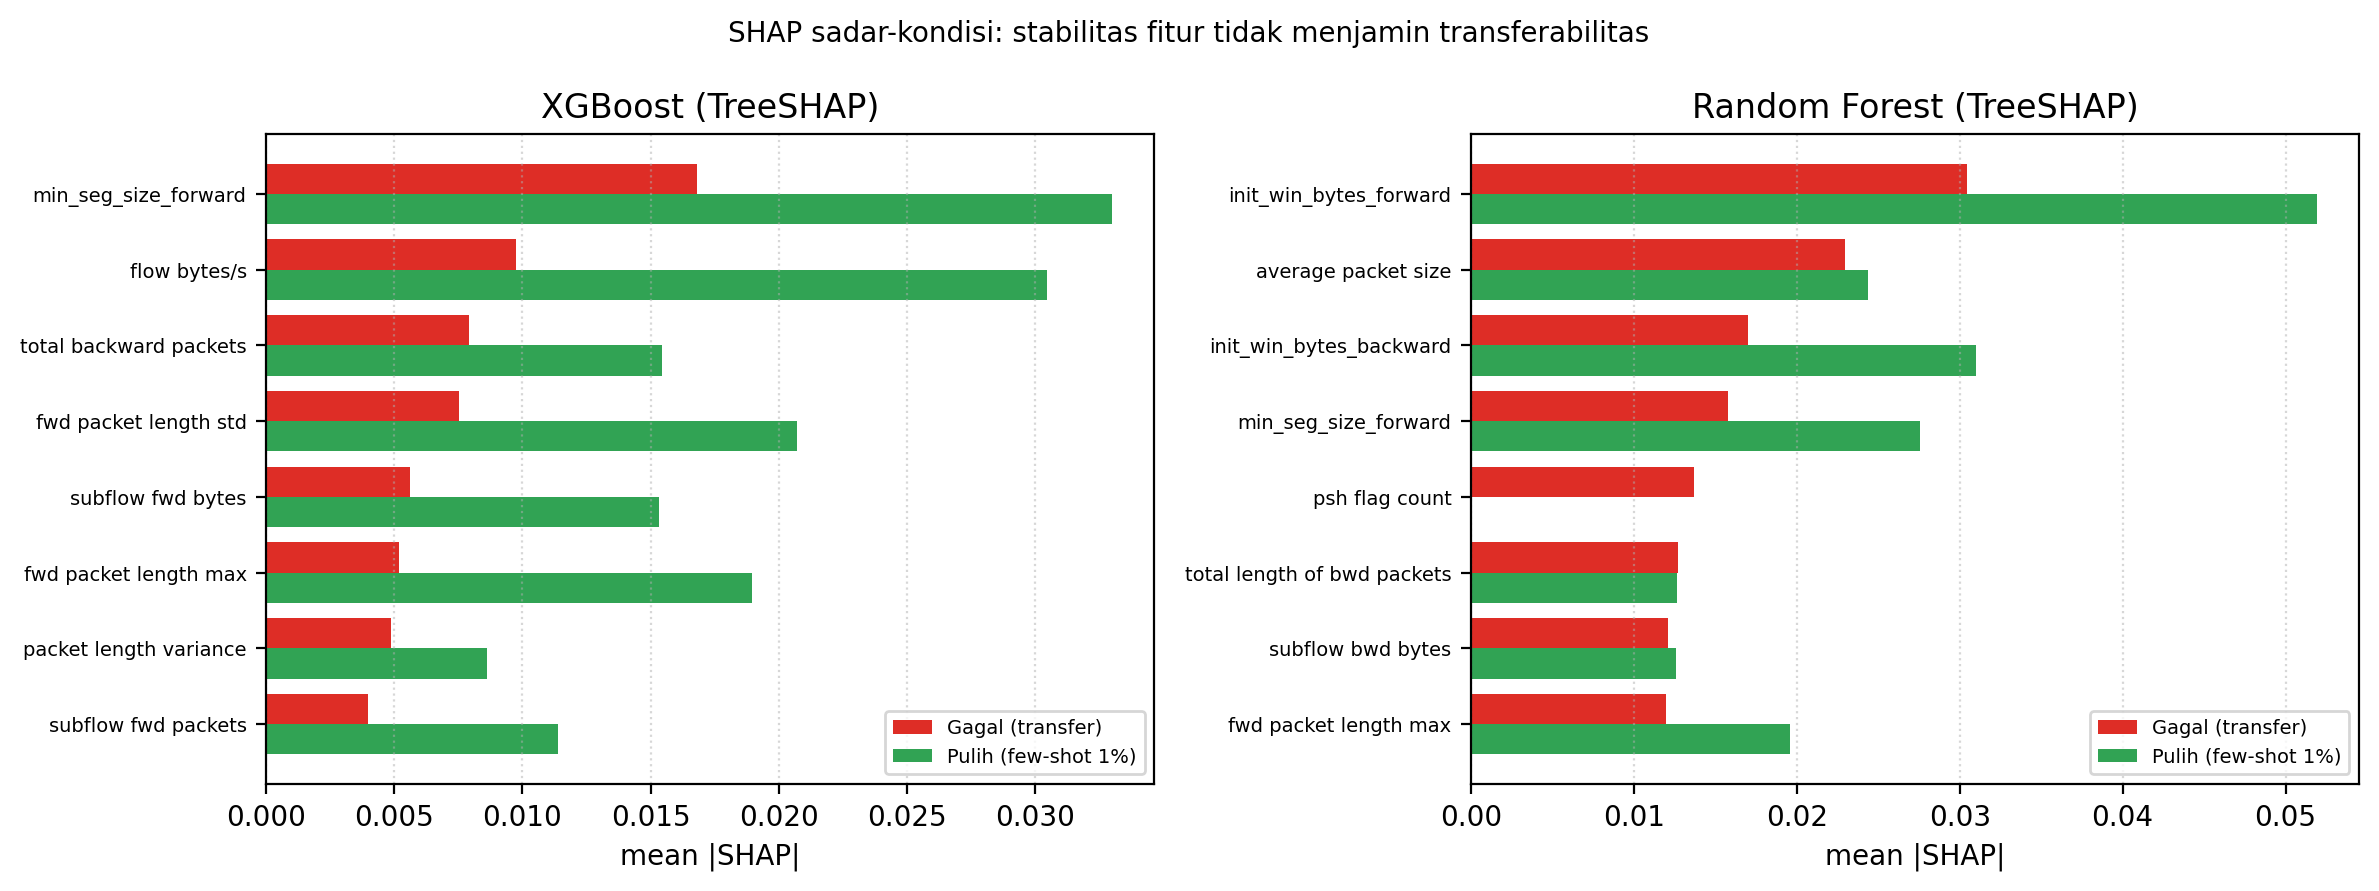
\includegraphics[width=0.9\textwidth]{figure-p4/fig4_shap.png}
\caption{Condition-aware SHAP feature importance (failed versus repaired model) for XGBoost
and Random Forest. Feature-ranking stability across conditions does not translate into
cross-dataset transferability.}
\label{fig:shap}
\end{figure}

\subsection{Multi-Seed Confidence and Limitations}
All headline numbers are means over 5 seeds $\{42,1,7,123,2024\}$ with 95\% $t$-intervals
($\mathrm{df}=4$); for example within CIC2017 MCC is $0.955\,[0.940,0.970]$ (XGBoost) and
$0.979\,[0.971,0.988]$ (RF), and cross CIC2017$\rightarrow$CIC2018 MCC@0.5 is
$0.067\,[0.012,0.122]$. Limitations: (i) binary classification only; (ii) two datasets from
a single extractor (CICFlowMeter), limiting generalization; (iii) each source file capped at
100{,}000 rows; (iv) direct quantification of distribution shift (e.g., per-feature
Wasserstein distance or domain-classifier accuracy) was not computed and is left to future
work --- the indirect evidence is the sharp within-vs-cross contrast and the changed optimal
threshold on the target; (v) XGBoost in the SHAP notebook uses an explicit
\texttt{base\_score}=0.5 for interpretability-library compatibility, which does not affect
performance metrics.

\subsection{Comparison with Predecessor Work}
This study is a direct continuation of the authors' predecessor manuscript \cite{martono},
which diagnosed cross-dataset generalization collapse. Table~\ref{tab:predecessor} makes the
added value explicit.

\begin{table}[htbp]
\centering
\caption{Position relative to the predecessor work.}
\label{tab:predecessor}
\footnotesize
\begin{tabular}{p{3.2cm}p{4.3cm}p{4.3cm}}
\toprule
Aspect & Predecessor (JTIIK) & This work \\
\midrule
Feature alignment & 75-feature harmonization with \textbf{zero-fill} for missing features & \textbf{Name intersection} (76 features), no zero-fill \\
Model & Random Forest (reference) & XGBoost \emph{and} Random Forest (identical protocol) \\
Cross MCC@0.5 (2017$\rightarrow$2018) & \textbf{0.00 across all 10 partitions} (attack recall 0) & 0.067 (XGB) / 0.175 (RF) --- collapsed but not absolute zero \\
Cross-dataset AUC & $\approx 0.46$ mean ($\approx$ chance) & 0.779 (XGB) --- above chance \\
Failure type & Read purely as distribution shift & \textbf{Separated}: ranking vs thresholding \\
Repair & None (stops at diagnosis) & \textbf{Threshold calibration + 1\% few-shot} (MCC up to 0.66--0.99) \\
Transfer direction & One-way (2017$\rightarrow$2018) & \textbf{Bidirectional} (2017$\leftrightarrow$2018) \\
SHAP & Computed on the failed model only & \textbf{Condition-aware} (failed vs repaired) and cross-model \\
\bottomrule
\end{tabular}
\end{table}

The most striking numeric difference---MCC of 0.00 with chance-level AUC in the predecessor
versus small-but-positive MCC with AUC 0.779 here---most likely stems from the
feature-alignment strategy. Zero-filling missing features in the predecessor injects
constant columns that can distort the decision boundary and mask the model's ranking
ability; the pure name-intersection approach here avoids that artifact, revealing that part
of the ``failure'' is in fact a thresholding problem that can be repaired. This work thus
does not merely reproduce the predecessor's finding but corrects its interpretation and
completes the recovery path that the predecessor only suggested as future work.

\section{Conclusion}
We diagnosed and repaired cross-dataset generalization failure for NIDS on a leakage-free
pipeline without semantic feature mapping, using CIC-IDS2017 (reference) and CSE-CIC-IDS2018
(target). Reference models reach high within-dataset performance (MCC 0.955 and 0.979) but
collapse under direct transfer (MCC@0.5 of 0.067 and 0.175, near-zero attack recall). Unlike
prior work, we separate ranking failure from thresholding failure --- threshold calibration
lifts XGBoost MCC to 0.498 (AUC 0.779) but Random Forest only to 0.403 (AUC 0.573) --- and we
repair detection with minimal few-shot calibration, where 1\% of target labels raises MCC to
0.663--0.969 depending on model and direction. Condition-aware SHAP (Spearman 0.72 between
failed and repaired, but only 0.20 between models) shows feature-ranking stability does not
guarantee transferability. Future work: quantifying distribution shift, heavier shift
scenarios (e.g., CIC-DDoS2019), multi-class classification, and live-traffic validation.

\section*{Acknowledgements}
The authors thank Politeknik Elektronika Negeri Surabaya (PENS) for support, and the AWS
partner for the cloud computing resources used in these experiments.

\begin{thebibliography}{99}
\bibitem{sharafaldin} I.~Sharafaldin, A.~H.~Lashkari, and A.~A.~Ghorbani, ``Toward generating a new intrusion detection dataset and intrusion traffic characterization,'' \emph{Proc. 4th ICISSP}, pp.~108--116, 2018.
\bibitem{buczak} A.~L.~Buczak and E.~Guven, ``A survey of data mining and machine learning methods for cyber security intrusion detection,'' \emph{IEEE Commun. Surveys Tuts.}, 18(2), pp.~1153--1176, 2016.
\bibitem{shone} N.~Shone, T.~N.~Ngoc, V.~D.~Phai, and Q.~Shi, ``A deep learning approach to network intrusion detection,'' \emph{IEEE Trans. Emerg. Topics Comput. Intell.}, 2(1), pp.~41--50, 2018.
\bibitem{wu} Z.~Wu, H.~Zhang, P.~Wang, and Z.~Sun, ``RTIDS: A robust transformer-based approach for intrusion detection system,'' \emph{IEEE Access}, 10, pp.~64375--64387, 2022.
\bibitem{dhooge} L.~D'Hooge, T.~Wauters, B.~Volckaert, and F.~De~Turck, ``Inter-dataset generalization strength of supervised machine learning methods for intrusion detection,'' \emph{J. Inf. Secur. Appl.}, 54, 102564, 2020.
\bibitem{cantone} M.~Cantone, C.~Marrocco, and A.~Bria, ``Machine learning in network intrusion detection: A cross-dataset generalization study,'' \emph{IEEE Access}, 12, pp.~144491--144509, 2024.
\bibitem{layeghygen} S.~Layeghy and M.~Portmann, ``On generalisability of machine learning-based network intrusion detection systems,'' \emph{Comput. Electr. Eng.}, 108, 108692, 2023.
\bibitem{kheddar} H.~Kheddar, Y.~Himeur, and A.~I.~Awad, ``Deep transfer learning applications in intrusion detection systems: A comprehensive review,'' \emph{arXiv:2304.10550}, 2023.
\bibitem{engelen} G.~Engelen, V.~Rimmer, and W.~Joosen, ``Troubleshooting an intrusion detection dataset: The CICIDS2017 case study,'' \emph{Proc. IEEE SPW}, pp.~7--12, 2021.
\bibitem{rosay} A.~Rosay, E.~Cheval, F.~Carlier, and P.~Leroux, ``Network intrusion detection: A comprehensive analysis of CIC-IDS2017,'' \emph{Proc. 8th ICISSP}, pp.~25--36, 2022.
\bibitem{lanvin} M.~Lanvin, P.-F.~Gimenez, Y.~Han, F.~Majorczyk, L.~M\'e, and \'E.~Totel, ``Errors in the CICIDS2017 dataset and the significant differences in detection performances it makes,'' \emph{Proc. CRiSIS}, pp.~18--33, 2022.
\bibitem{liu} L.~Liu, G.~Engelen, T.~Lynar, D.~Essam, and W.~Joosen, ``Error prevalence in NIDS datasets: A case study on CIC-IDS-2017 and CSE-CIC-IDS-2018,'' \emph{Proc. IEEE CNS}, pp.~254--262, 2022.
\bibitem{catillo} M.~Catillo, A.~Pecchia, and U.~Villano, ``Machine learning on public intrusion datasets: Academic hype or concrete advances in NIDS?,'' \emph{Proc. IEEE/IFIP DSN-S}, pp.~132--136, 2023.
\bibitem{layeghy} S.~Layeghy, M.~Gallagher, and M.~Portmann, ``Benchmarking the benchmark---Comparing synthetic and real-world network IDS datasets,'' \emph{J. Inf. Secur. Appl.}, 80, 103689, 2024.
\bibitem{martono} H.~Y.~Martono, I.~Syarif, and F.~A.~Saputra, ``Cross-dataset generalization of ML-based network intrusion detection via semantic feature mapping and few-shot adaptation, validated on real cloud traffic,'' manuscript (authors' predecessor work), 2024.
\bibitem{lundberg} S.~M.~Lundberg and S.-I.~Lee, ``A unified approach to interpreting model predictions,'' \emph{NeurIPS}, 30, pp.~4765--4774, 2017.
\bibitem{ribeiro} M.~T.~Ribeiro, S.~Singh, and C.~Guestrin, ```Why should I trust you?': Explaining the predictions of any classifier,'' \emph{Proc. 22nd ACM SIGKDD}, pp.~1135--1144, 2016.
\bibitem{arreche} O.~Arreche, T.~R.~Guntur, J.~W.~Roberts, and M.~Abdallah, ``XAI-IDS: Toward an explainable AI framework for network intrusion detection systems,'' \emph{Applied Sciences}, 14(10), 4170, 2024.
\bibitem{gaspar} D.~Gaspar, P.~Silva, and C.~Silva, ``Explainable AI for intrusion detection systems: LIME and SHAP applicability on multi-layer perceptron,'' \emph{IEEE Access}, 12, pp.~30164--30175, 2024.
\bibitem{wang} H.~Wang, J.~Li, and Y.~Zhang, ``Explainable deep learning for network intrusion detection using SHAP,'' \emph{Computers and Security}, 138, 103651, 2024.
\bibitem{mohale} V.~Z.~Mohale and I.~C.~Obagbuwa, ``A systematic review of explainable artificial intelligence in intrusion detection systems,'' \emph{Frontiers in AI}, 8, 1526221, 2025.
\bibitem{alabbaadi} A.~Alabbaadi and F.~Bajaber, ``IDS over IoT data streams using explainable AI,'' \emph{Sensors}, 25(3), 847, 2025.
\bibitem{layeghydi} S.~Layeghy, M.~Baktash, and M.~Portmann, ``DI-NIDS: Domain invariant network intrusion detection system,'' \emph{Knowledge-Based Systems}, 273, 110626, 2023.
\bibitem{sarhan} M.~Sarhan, S.~Layeghy, and M.~Portmann, ``Towards a standard feature set for network intrusion detection system datasets,'' \emph{Mobile Netw. Appl.}, 27(1), pp.~357--370, 2022.
\bibitem{chawla} N.~V.~Chawla, K.~W.~Bowyer, L.~O.~Hall, and W.~P.~Kegelmeyer, ``SMOTE: Synthetic minority over-sampling technique,'' \emph{J. Artif. Intell. Res.}, 16, pp.~321--357, 2002.
\bibitem{pedregosa} F.~Pedregosa et al., ``Scikit-learn: Machine learning in Python,'' \emph{J. Mach. Learn. Res.}, 12, pp.~2825--2830, 2011.
\bibitem{breiman} L.~Breiman, ``Random forests,'' \emph{Machine Learning}, 45(1), pp.~5--32, 2001.
\bibitem{chen} T.~Chen and C.~Guestrin, ``XGBoost: A scalable tree boosting system,'' \emph{Proc. 22nd ACM SIGKDD}, pp.~785--794, 2016.
\bibitem{ke} G.~Ke, Q.~Meng, T.~Finley, T.~Wang, W.~Chen, W.~Ma, Q.~Ye, and T.-Y.~Liu, ``LightGBM: A highly efficient gradient boosting decision tree,'' \emph{NeurIPS}, 30, pp.~3146--3154, 2017.
\bibitem{husain} A.~Husain, A.~Salem, C.~Jim, and G.~Dimitoglou, ``Development of an efficient network intrusion detection model using XGBoost on the UNSW-NB15 dataset,'' \emph{Proc. IEEE ISSPIT}, pp.~1--7, 2019.
\bibitem{moustafa15} N.~Moustafa and J.~Slay, ``UNSW-NB15: A comprehensive data set for network intrusion detection systems,'' \emph{Proc. MilCIS}, pp.~1--6, 2015.
\bibitem{moustafa16} N.~Moustafa and J.~Slay, ``The evaluation of network anomaly detection systems: Statistical analysis of the UNSW-NB15 data set and the comparison with the KDD99 data set,'' \emph{Inf. Secur. J.}, 25(1--3), pp.~18--31, 2016.
\bibitem{chicco} D.~Chicco and G.~Jurman, ``The advantages of the Matthews correlation coefficient (MCC) over F1 score and accuracy in binary classification evaluation,'' \emph{BMC Genomics}, 21(1), 6, 2020.
\bibitem{verkerken} M.~Verkerken, L.~D'Hooge, T.~Wauters, B.~Volckaert, and F.~De~Turck, ``Towards model generalization for intrusion detection: Unsupervised machine learning techniques,'' \emph{J. Netw. Syst. Manage.}, 30(1), pp.~1--25, 2022.
\bibitem{sun} B.~Sun and K.~Saenko, ``Deep CORAL: Correlation alignment for deep domain adaptation,'' \emph{Proc. ECCV Workshops}, pp.~443--450, 2016.
\bibitem{molnar} C.~Molnar, \emph{Interpretable Machine Learning: A Guide for Making Black Box Models Explainable}, 2nd ed., 2022.
\end{thebibliography}

\end{document}
